%-%-%-%-%-%-%-%-%-%-%-%-%-%-%-%-%-%-%-%-%-%-%-%-%-%
% EE531: laboratório de Eletrônica Básica I       %  
% Experimento 2: Diodos                           %
% Data:20/08/2010                                 %
% Unicamp,Campinas,São Paulo,Brasil               % 
% Grupo:                                          %
%       - Daniel Lins Mattos                      %
%       - Raquel Mayumi Kawamoto                  %
%       - Tiago Chedraoui Silva                   % 
%-%-%-%-%-%-%-%-%-%-%-%-%-%-%-%-%-%-%-%-%-%-%-%-%-%
%\documentclass[letter]{article}  % formato impressao IC
\documentclass[a4paper]{article} % formato impressao FEEC

%%% fontes %%%
\usepackage[T1]{fontenc}
\usepackage[brazil]{babel}    % dá suporte para os termos na língua portuguesa do Brasi
\usepackage[utf8]{inputenc}   % acentuação
\usepackage{ae,aecompl,aeguill}       % pdfs mais bonitos =)

%%% outros %%%
\usepackage{multirow}
\usepackage{textcomp}
\usepackage{color}       
\usepackage{indentfirst}      % retira padrao americano de paragrafos
\usepackage{multicol}   
\usepackage[linkbordercolor={1 1 1},urlcolor=black,colorlinks=true]{hyperref} % links
\usepackage{subfig}
\usepackage[letterpaper]{geometry}
\geometry{verbose,lmargin=3cm,rmargin=3cm}

% circuito eletrico
\usepackage{electComp}
\usetikzlibrary{decorations,decorations.pathmorphing,decorations.pathreplacing}
\usepackage{verbatim}
\usepackage{pstricks}
\usepackage{boxdims}

\setcounter{tocdepth}{0}

\renewcommand{\thefigure}{\arabic{figure}}

\date{Outubro 1, 2010}
% Capa estilizada %
\newcommand*{\titleTMB}{\begingroup \centering \settowidth{\unitlength}{\LARGE EE531} {\large\scshape EE531 - Turma S}\\[0.2\baselineskip] \rule{11.0cm}{1.6pt}\vspace*{-\baselineskip}\vspace*{2pt} \rule{11.0cm}{0.4pt}\\[\baselineskip] {\LARGE Transistores bipolares}\\\vspace*{\baselineskip}  {\itshape Laboratório de Eletrônica Básica I - Segundo Semestre de 2010}\\ \rule{11.0cm}{0.4pt}\vspace*{-\baselineskip}\vspace{3.2pt} \rule{11.0cm}{1.6pt}\\[\baselineskip] {\large\scshape Professor: José Cândido Silveira Santos Filho}\par \vfill {\normalsize   \scshape 
    \begin{center} 
      \begin{tabular}{  l  l  p{5cm} } 
 	Daniel Lins Mattos & RA: 059915\\
        Raquel Mayumi Kawamoto & RA: 086003\\
        Tiago Chedraoui Silva  & RA: 082941\\
      \end{tabular} \end{center}
    \itshape 1 de outubro de 2010    }\\[\baselineskip] \vspace{3.2pt} \endgroup}


\begin{document}
\titleTMB 
\newpage

Para o presente experimento, tem-se como objetivo o estudo dos transistores bipolares, em
especial o de configuração emissor comum. Para tal, realizar-se-ão o cálculo do ponto de
operação, a análise para pequenos sinais, os efeitos da temperatura nas características da
configuração emissor comum e a verificação da estabilidade do ponto de operação e do
ganho.

Para tal experimento, foram utilizados um resistor, podendo ser de valor 470$\Omega$, 1.2k$\Omega$, 5.1k$\Omega$,
15k$\Omega$, 100k$\Omega$, 560k$\Omega$, 750k$\Omega$; um trimpot (20 voltas, de 10k$\Omega$), um capacitor de 1$\mu$F e um
transistor bipolar NPN, BC548.

\section*{Parte Experimental}

Inicialmente, com um multímetro adequado, foi medido o ganho de corrente DC
($\beta_{cc}$)do transistor bipolar. Esta medição resultou em um valor de ganho de corrente
$\beta_{cc}$=295.


Em seguida, analisando-se o circuito de um amplificador na configuração emissor
comum, da figura 1, foi calculado o valor da resistor
para que se tenha uma tensão no
coletor de $V_c=$8V. Fazendo-se os cálculos, chega-se a um valor de resistência
$R_{B1}=723k\Omega$.
\begin{displaymath}
I_C=\frac{15-8}{1.2k}=5.83mA
\end{displaymath}
\begin{displaymath}
I_B=\frac{I_C}{1.2k}=19.77\mu A
\end{displaymath}

\begin{figure}[h]
\centerline{\input circ2.tex}
\caption{Circuito 1\label{circ:1}}
\end{figure}


Considerando-se que a tensão $V_{BE}=0.7V$ 
, então a tensão de $V_{B}=0.7V$ , já que o
emissor está aterrado. Portanto, a resistência
$R_{B1}=\frac{15-7}{I_B}=723.3k\Omega$.


Feita esta análise teórica, foi utilizado um multímetro para medir o valor de $R_C$ e de $R_{B1}$. As medidas encontradas foram, para cada resistência, respectivamente de $1,15k\Omega$ e $557k\Omega$. A seguir, foi montado o circuito da figura 1, na qual obteve-se um $V_C=5.61V$ e um $V_B=0.67V$. Calculando-se $I_C$, $I_B$ e $\beta$ obteve-se, respectivamente, $I_C=8.16mA$, $I_B=25.72\mu A$ e $\beta=317.5$. Ou seja, estes são os valores experimentais.

Calculando-se usando valores teóricos, na qual $V_C=8V$, $V_B=0.7V$ e $R_C=1.2k\Omega$ tem-se para  $I_C=5.83mA$, $I_B=19.77\mu A$ e $\beta=294.89$.

Feita a análise DC do circuito da figura 1, é feita agora uma análise de pequenos sinais para o mesmo. Para esta etapa, são calculadas (1) a impedância de entrada $R_{in}$ do circuito, (2) a freqüência de passagem determinada por $C_C$ e $R_{in}$ , (3) a transcondutância do bipolar operando nesta condição e o (4) ganho ($\frac{v_c}{v_{in}}$).


%\setcounter{figure}{0}

\vspace{3mm}


\begin{eqnarray}
R_{in}=R_{B1}||r_{\pi}\\
f_c=\frac{1}{2\pi C_cR_{in}}\\
g_m=\frac{I_c}{V_T},sendo \; V_T = 25 mV\\
A_v=-g_mR_C\\
r_{\pi}=\frac{\beta}{g_m}
\end{eqnarray}


Os valores, tanto teórico quanto experimental, calculados para tais medidas da análise
de pequenos sinais encontram-se na tabela abaixo.
\begin{table}[h!]
\begin{centering}
\begin{tabular}{ccc}
\hline 
 & Valor teórico & Valor experimental\tabularnewline
\hline
\hline 
$R_{in}$ & 1261.67$\Omega$ & 971.04$\Omega$\tabularnewline
$f_{c}$ & 126.15 Hz & 163.90 Hz\tabularnewline
$g_{m}$ & 0.23 A/V & 0.32 A/V\tabularnewline
$A_{v}$ & -268.18 V/V & -375.36 V/V\tabularnewline
$r_{\pi}$ & 1264.53$\Omega$ & 972.73$\Omega$\tabularnewline
\hline
\end{tabular}
\par\end{centering}

\caption{Dados calculados circuito 1}

\end{table}


Aplicando um sinal de 10mVp (offset = 0 e freqüência = 10kHz) na entrada
$v_{in}$ do circuito através do capacitor de acoplamento, encontra-se o ganho experimental, na
qual seu valor é de $A_v=243.3 V/V$. A tensão $v_{in}=24.0mV$ e $v_c=5.84V$
e o ganho é de $\frac{v_c}{v_{in}}$.

%\newpage
\begin{figure}[h!]
\begin{centering}
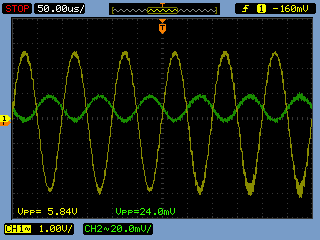
\includegraphics[scale=0.5]{figuras03/1_1} \caption{Sinal de entrada e saída do circuito 1 \label{fig:11}}
\par\end{centering}
\end{figure}

Feita a etapa anterior, continua-se monitorando constantemente o sinal do coletor
com o osciloscópio enquanto o transistor é aquecido com o ferro de soldar e observa-se qual o
efeito da temperatura tanto no ganho da tensão quanto no valor da tensão cc do coletor ($V_c$).

Aquecendo-se o transistor no circuito da figura 1, percebe-se que a tensão do coletor
cai consideravelmente, o que nos leva a concluir que o ganho aumenta, a transcondutância
($g_m$) aumenta e $I_C$ aumenta também.

Para o circuito 1 a análise já está terminada, passando-se assim para a análise do
circuito da figura 3.

\vspace{3mm}
\begin{figure}[h!]
\centerline{\input circ1.tex}
\caption{Circuito 2\label{circ:2}}
\end{figure}

Para a montagem do circuito 2, desconectou-se o gerador de sinais e foi introduzido
um resistor de emissor ($R_E$) no circuito, como ilustra o circuito da figura 3. Novamente,
recalcula-se o valor de $R_{B1}$, porém para o circuito 2.

\begin{displaymath}
I_c=\frac{15-V_C}{R_c}=\frac{15-8}{1.2k}\cong5.83mA
\end{displaymath}

\begin{displaymath}
I_E=\frac{\beta +1}{\beta}I_c=\frac{296}{295}5.83mA\cong5.85mA
\end{displaymath}

\begin{displaymath}
V_E=R_EI_E=470\Omega 5.85mA \cong 2.75V
\end{displaymath}
\begin{displaymath}
V_B=V_E+0.7=3.45V
\end{displaymath}
\begin{displaymath}
I_B=\frac{I_C}{\beta}=\frac{5.83mA}{295}=19.76\mu A
\end{displaymath}

\begin{displaymath}
R_{B1}=\frac{15-V_B}{I_B}=\frac{14-3.45}{19.76\mu A} \cong 584.5k\Omega 
\end{displaymath}

Os valores teóricos para as tensões $V_B$,$V_C$ e $V_E$ e para as correntes $I_B$,$I_C$ e $I_E$
são respectivamente,$V_B=3.45V$, $V_C=8.0V$, $V_E=2.75V$, $I_B=19.76 \mu A$,$I_C=5.83mA$ e $I_E=5.85mA$.
O ganho experimental é de $\beta =295.04$ . 

Encontrado o valor de $R_{B1}$, usa-se uma resistência de $560k\Omega$
experimental e medem-se as tensões $V_B$,$V_C$ e $V_E$  e as correntes $I_B$,$I_C$ e $I_E$.Com um
multímetro, calculou-se $V_B$,$V_C$ e $V_E$. Seus respectivos valores são $V_B=3.89V$,$V_C=8.27V$
e $V_E=2.91V$.


\begin{displaymath}
I_c=\frac{15-V_C}{R_c}=\frac{15-8.27}{1.2k}\cong5.85mA
\end{displaymath}


\begin{displaymath}
I_B=\frac{15-V_B}{R_{B1}}=\frac{15-3.89}{557k}=19.95\mu A
\end{displaymath}


\begin{displaymath}
I_E=I_B+I_C \cong 5.85mA
\end{displaymath}

\begin{displaymath}
\beta_{CC}=\frac{I_C}{I_B}=293.23
\end{displaymath}

%Aplicando um sinal de 10mVp (offset = 0 e freqüência = 10kHz) na entrada
%do $v_{in}$ circuito 2 através do capacitor de acoplamento, encontra-se o ganho experimental, na
%qual seu valor é de $A_v 2.43 V/V$. A tensão $v_{in}= 46.0mV$ e $v_c=112mV$ e o ganho
%é de $A_v=\frac{v_c}{v_in}$.

Foi feita analise de pequenos sinais também para o circuito da figura 3.


\begin{eqnarray}
R_{in}=R_{B1}||(\beta+1)(r_{e}+R_E)\\
f_c=\frac{1}{2\pi C_cR_{in}}\\
g_m=\frac{I_c}{V_T},sendo \; V_T = 25 mV\\
A_v=\frac{-g_mR_C}{1+g_mR_e}\\
r_{e}=\frac{\beta}{(\beta+1)g_m}
\end{eqnarray}

Os valores, tanto teórico quanto experimental, calculados para tais medidas da análise
de pequenos sinais encontram-se na tabela abaixo.

\begin{table}[h!]
\begin{centering}
\begin{tabular}{ccc}
\hline 
 & Valor teórico & Valor experimental\tabularnewline
\hline
\hline 
$R_{in}$ & 112.80$k\Omega$ & 111.30$k\Omega$\tabularnewline
$f_{c}$ & 1.41 Hz & 1.43 Hz\tabularnewline
$g_{m}$ & 0.23 A/V & 0.23 A/V\tabularnewline
$A_{v}$ & -2.54 V/V & -2.54 V/V\tabularnewline
\hline
\end{tabular}
\par\end{centering}

\caption{Dados calculados circuito 2}

\end{table}
%
Aplicando um sinal de $10mV_p$(offset = 0 e freqüência = 10kHz) na entrada $v_{in}$
do circuito 2 através do capacitor de acoplamento, encontra-se o ganho experimental, na qual seu
valor é de $A_v=2.43V/V$. A tensão $v_{in}=46mV$ e $v_c=122mV$ e o ganho é de  $A_v=\frac{v_c}{v_{in}}$.

%%%%%%%%%%%%%%TDDOODOODODODOD
Aquecendo-se o transistor no circuito 2, percebe-se que a tensão do coletor
cai, havendo um aumento de $I_C$, mas devido a existência do $R_E$, tanto $V_E$ quanto $I_E$ aumentam. Portanto, $I_C$ é induzido a uma estabilização.
Assim, o circuito possui certa estabilidade quanto ao ponto de operação.

\begin{figure}[h!]
\begin{centering}
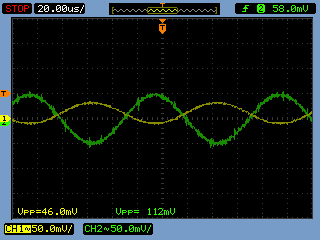
\includegraphics[scale=0.5]{figuras03/2} \caption{Sinal de entrada e saída do circuito 2 \label{fig:3}}
\par\end{centering}
\end{figure}

\newpage


Em seguida, foi desconectado o gerador de sinais e substituiu-se o $R_{B1}=15k\Omega$
e introduziu-se o trimpot ($R_{B2}$) no circuito, gerando o circuito da figura 4. Feito isto,
como o trimpot é um resistor de resistência variável, ele foi ajustado, alterando o
ponto de operação do circuito de forma a se obter a máxima excursão de sinal de saída
$V_C=8.0V$. O valor de $R_{B2}$ ajustado é de $R_{B2}=4.73k\Omega$.

Com este valor de $R_{B2}=4.73k\Omega$, foi medido os valores de
$V_B=3.5V$,$V_C=8.02V$ e $V_E=2.85V$. E o valor medido de $R_E$ é $R_E =467.9\Omega$.

Calcula-se, para os valores de resistência obtidos através das medidas indicados, os
valores de corrente pedidos:

\begin{displaymath}
I_C =\frac{(15-8.02)}{1.15K} = 6.07 mA
\end{displaymath}

\begin{displaymath}
I_E =\frac{2.85}{467.9} = 6.09 mA
\end{displaymath}

\begin{displaymath}
I_B = I_E - I_C = 20 \mu A
\end{displaymath}

Nesse caso $\beta = \frac{I_C}{I_B} = 303.5$, que é um valor próximo do valor medido no início do
experimento.


\vspace{3mm}
\begin{figure}[h!]
\centerline{\input circ3.tex}
\caption{Circuito 3\label{circ:3}}
\end{figure}


Para este circuito 3, também foi feita analise de pequenos sinais.
\begin{eqnarray}
R_{in}=R_{B1}||R_{B2}||(\beta+1)(r_{e}+R_E)\\
f_c=\frac{1}{2\pi C_cR_{in}}\\
g_m=\frac{I_c}{V_T},sendo \; V_T = 25 mV\\
A_v=\frac{-g_mR_C}{1+g_mR_e}\\
r_{e}=\frac{\beta}{(\beta+1)g_m}
\end{eqnarray}


%
Os valores, tanto teórico quanto experimental, calculados para tais medidas da análise
de pequenos sinais encontram-se na tabela abaixo.
\begin{table}[h!]
\begin{centering}
\begin{tabular}{ccc}
\hline 
 & Valor teórico & Valor experimental\tabularnewline
\hline
\hline 
$R_{in}$ & 4539.64$\Omega$ & 3505.31$\Omega$\tabularnewline
$f_{c}$ & 35.0 Hz & 45.40 Hz\tabularnewline
$g_{m}$ & 0.23 A/V & 0.23 A/V\tabularnewline
$A_{v}$ & -2.54 V/V & -2.54 V/V\tabularnewline
\hline
\end{tabular}
\par\end{centering}

\caption{Dados calculados circuito 3}

\end{table}



Aplicando um sinal de $10mV_p$ (offset = 0 e freqüência = 10kHz) na entrada $v_{in}$
do circuito 3 através do capacitor de acoplamento, encontra-se o ganho experimental, na qual seu
valor é de $A_v=2.43V/V$. A tensão  $v_{in}=46.0mV$ e  $v_c=112mV$ e o ganho é de $A_v=\frac{v_c}{v_{in}}$.


%\newpage
\begin{figure}[h!]
\begin{centering}
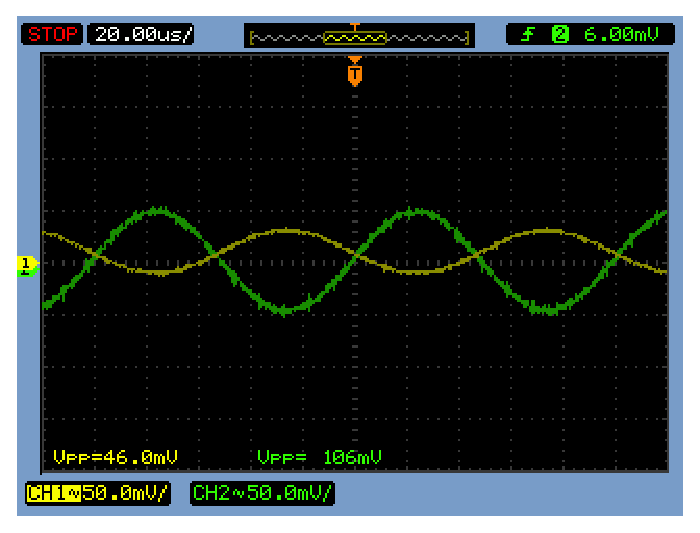
\includegraphics[scale=0.5]{figuras03/3} \caption{Sinal de entrada e saída do circuito 3 \label{fig:2}}
\par\end{centering}
\end{figure}

Aquecendo-se o transistor no circuito da figura 5, percebe-se que o circuito é quase
estável quanto ao ponto de operação e ao ganho de tensão. A tensão no coletor vai
diminuindo gradualmente e quando atinge uma tensão aproximada de 7.5V,
se establiza.
Como o aquecimento do transistor, $V_{pp}$ também diminiu, estabilizando em 100mV,
aproximadamente.



%\begin{figure}[h]
%\begin{centering}
%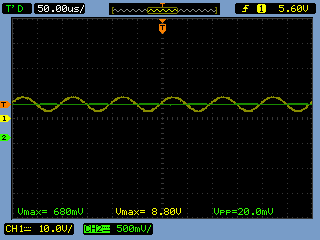
\includegraphics[scale=0.7]{figuras03/1} \caption{Nome fig 1 \label{fig:1}}
%\par\end{centering}
%\end{figure}


%\newpage
%\begin{figure}[h]
%\begin{centering}
%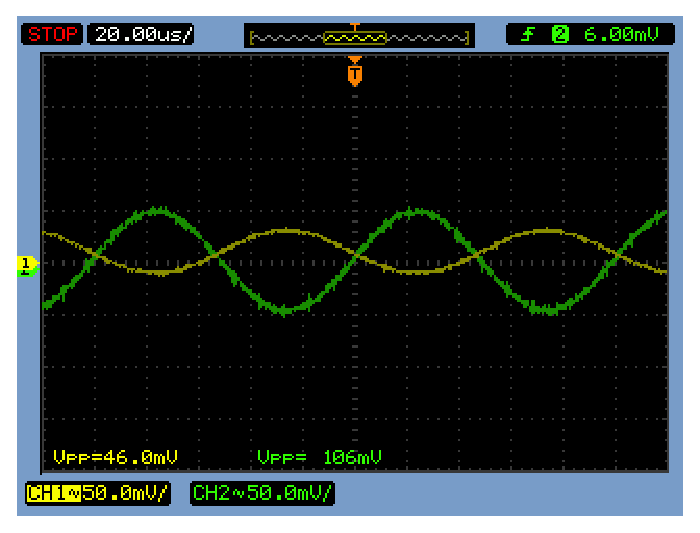
\includegraphics[scale=0.7]{figuras03/3} \caption{Nome fig 2 \label{fig:2}}
%\par\end{centering}
%\end{figure}





%\newpage

%\begin{figure}[h]
%\begin{centering}
%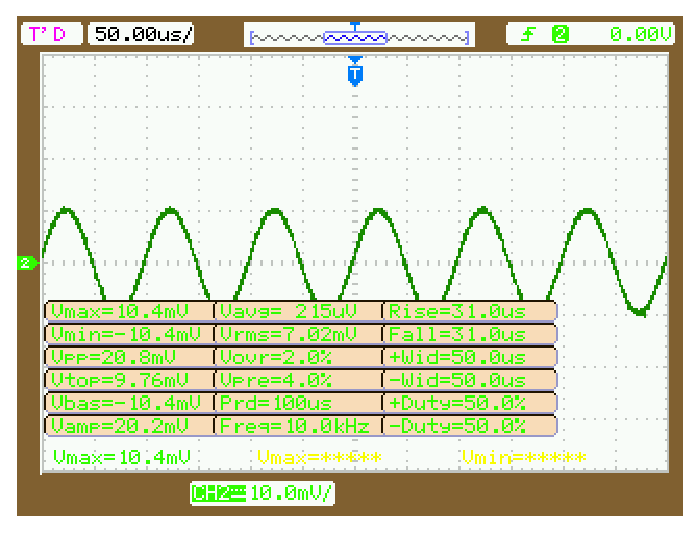
\includegraphics[scale=0.7]{figuras03/4} \caption{Nome fig 4 \label{fig:4}}

%\par\end{centering}
%\end{figure}


\section*{Conclusão}


Como foi possível verificar durante o experimento os valores teóricos foram compatíveis com os valores obtidos na prática, como os valores de $\beta$ que foram próximos daquele medido com o multímetro.

Foi interessante observar também a validade da análise de pequenos sinais para os três amplificadores emissor comum tratados na experiência. 

Finalmente, o efeito da temperatura nos transistores TBJ foi também comprovado. Isso mostra a capacidade do TBJ de ser aplicado, por exemplo, em sensores de térmicos, mas também é um aviso que o engenheiro deve prestar atenção nas condições de temperatura nas quais o seu sistema será aplicado, pois com a variação de temperatura o TBJ pode sair da zona de operação desejada. 




\end{document}
